\hypertarget{exploring-distributions}{%
\chapter{Exploring Distributions}\label{exploring-distributions}}

\hypertarget{introduction}{%
\section{Introduction}\label{introduction}}

This is the second in a series of notebooks that make up a
\href{https://allendowney.github.io/PoliticalAlignmentCaseStudy/}{case
study in exploratory data analysis}. This case study is part of the
\href{https://allendowney.github.io/ElementsOfDataScience/}{\emph{Elements
of Data Science}} curriculum.

In this notebook, we:

\begin{enumerate}
\def\labelenumi{\arabic{enumi}.}
\item
  Look at responses to the variable \passthrough{\lstinline!polviews!},
  which represent political alignment on a 7-point scale from liberal to
  conservative.
\item
  Compare the distribution of responses in 1974 and 1990.
\item
  Plot the mean and standard deviation of responses over time as a way
  of quantifying changes in political alignment and polarization.
\item
  Use local regression to plot a smooth line through noisy data.
\item
  Use cross tabulation to compute the fraction of respondents in each
  category over time.
\item
  Plot the results using a custom color palette.
\end{enumerate}

As an exercise, you will look at changes in political party affiliation
over the same period.

The following cell installs the \passthrough{\lstinline!empiricaldist!}
library if necessary.

\begin{lstlisting}[language=Python,style=source]
try:
    import empiricaldist
except ImportError:
    !pip install empiricaldist
\end{lstlisting}

If everything we need is installed, the following cell should run
without error.

\begin{lstlisting}[language=Python,style=source]
import pandas as pd
import numpy as np
import matplotlib.pyplot as plt
import seaborn as sns

from empiricaldist import Pmf
\end{lstlisting}

The following cell defines a function I use to decorate the axes in
plots.

\begin{lstlisting}[language=Python,style=source]
def decorate(**options):
    """Decorate the current axes.
    
    Call decorate with keyword arguments like
    decorate(title='Title',
             xlabel='x',
             ylabel='y')
             
    The keyword arguments can be any of the axis properties
    https://matplotlib.org/api/axes_api.html
    """
    ax = plt.gca()
    ax.set(**options)
    
    handles, labels = ax.get_legend_handles_labels()
    if handles:
        ax.legend(handles, labels)

    plt.tight_layout()
\end{lstlisting}

\hypertarget{loading-the-data}{%
\section{Loading the data}\label{loading-the-data}}

In the previous notebook, we downloaded GSS data, loaded and cleaned it,
resampled it to correct for stratified sampling, and then saved the data
in an HDF5 file, which is much faster to load. In this and the following
notebooks, we'll download the HDF5 file and load it.

The following cell downloads the file if necessary.

\begin{lstlisting}[language=Python,style=source]
from os.path import basename, exists

def download(url):
    filename = basename(url)
    if not exists(filename):
        from urllib.request import urlretrieve
        local, _ = urlretrieve(url, filename)
        print('Downloaded ' + local)

download('https://github.com/AllenDowney/PoliticalAlignmentCaseStudy/' +
         'raw/master/gss_eda.3.hdf5')
\end{lstlisting}

This file contains three DataFrames containing resamples of the GSS
data. We'll work with the first resampling,
\passthrough{\lstinline!gss0!}, to get started; at the end of this
notebook, we'll see the other two as well.

\begin{lstlisting}[language=Python,style=source]
datafile = 'gss_eda.3.hdf5'
gss = pd.read_hdf(datafile, 'gss0')
gss.shape
\end{lstlisting}

\begin{lstlisting}[style=output]
(64814, 169)
\end{lstlisting}

\hypertarget{political-alignment}{%
\section{Political alignment}\label{political-alignment}}

The people surveyed as part of the GSS were asked about their
``political alignment'', which is where they place themselves on a
spectrum from liberal to conservative.

The variable \passthrough{\lstinline!polviews!} contains responses to
the
\href{https://gssdataexplorer.norc.org/projects/52787/variables/178/vshow}{following
question}:

\begin{quote}
We hear a lot of talk these days about liberals and conservatives. I'm
going to show you a seven-point scale on which the political views that
people might hold are arranged from extremely liberal--point 1--to
extremely conservative--point 7. Where would you place yourself on this
scale?
\end{quote}

Here are the valid responses:

\begin{lstlisting}[style=output]
1   Extremely liberal
2   Liberal
3   Slightly liberal
4   Moderate
5   Slightly conservative
6   Conservative
7   Extremely conservative
\end{lstlisting}

To see how the responses have changed over time, we'll inspect them at
the beginning and end of the observation period.

First I'll select the column.

\begin{lstlisting}[language=Python,style=source]
polviews = gss['polviews']
\end{lstlisting}

Then compute a Boolean Series that's \passthrough{\lstinline!True!} for
responses from 1974.

\begin{lstlisting}[language=Python,style=source]
year74 = (gss['year'] == 1974)
\end{lstlisting}

Now we can select the responses from 1974.

\begin{lstlisting}[language=Python,style=source]
polviews74 = polviews[year74]
\end{lstlisting}

As in the previous notebook, we'll use \passthrough{\lstinline!values!}
to plot the values in the series and their frequencies.

\begin{lstlisting}[language=Python,style=source]
def values(series):
    """Count the values and sort.
    
    series: pd.Series
    
    returns: series mapping from values to frequencies
    """
    return series.value_counts().sort_index()
\end{lstlisting}

Here are the responses from 1974.

\begin{lstlisting}[language=Python,style=source]
values(polviews74)
\end{lstlisting}

\begin{tabular}{lr}
\toprule
{} &  polviews \\
\midrule
1.0 &        31 \\
2.0 &       201 \\
3.0 &       211 \\
4.0 &       538 \\
5.0 &       223 \\
6.0 &       181 \\
7.0 &        30 \\
\bottomrule
\end{tabular}

And here are the responses from 2018.

\begin{lstlisting}[language=Python,style=source]
year18 = (gss['year'] == 2018)
polviews18 = polviews[year18]
values(polviews18)
\end{lstlisting}

\begin{tabular}{lr}
\toprule
{} &  polviews \\
\midrule
1.0 &        89 \\
2.0 &       269 \\
3.0 &       265 \\
4.0 &       891 \\
5.0 &       310 \\
6.0 &       342 \\
7.0 &        92 \\
\bottomrule
\end{tabular}

\hypertarget{pmfs}{%
\section{PMFs}\label{pmfs}}

To visualize these distributions, we'll use the Probability Mass
Function (PMF), which is similar to a histogram. The difference is that
the PMF is ``normalized'', which means that it shows the percentage of
people who gave each response, rather than the number.

I'll use the \passthrough{\lstinline!Pmf!} class from
\passthrough{\lstinline!empiricaldist!} to compute them.

\begin{lstlisting}[language=Python,style=source]
from empiricaldist import Pmf
\end{lstlisting}

Here's the distribution from 1974:

\begin{lstlisting}[language=Python,style=source]
pmf74 = Pmf.from_seq(polviews74)
pmf74.bar(label='1974', color='C0', alpha=0.7)

decorate(xlabel='Political view on a 7-point scale',
         ylabel='Fraction of population',
         title='Distribution of political views')
\end{lstlisting}

\begin{center}
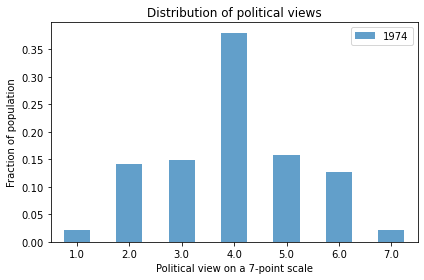
\includegraphics[scale=0.75]{02_polviews_files/02_polviews_30_0.png}
\end{center}

And from 2018:

\begin{lstlisting}[language=Python,style=source]
pmf18 = Pmf.from_seq(polviews18)
pmf18.bar(label='2018', color='C1', alpha=0.7)

decorate(xlabel='Political view on a 7-point scale',
         ylabel='Fraction of population',
         title='Distribution of political views')
\end{lstlisting}

\begin{center}
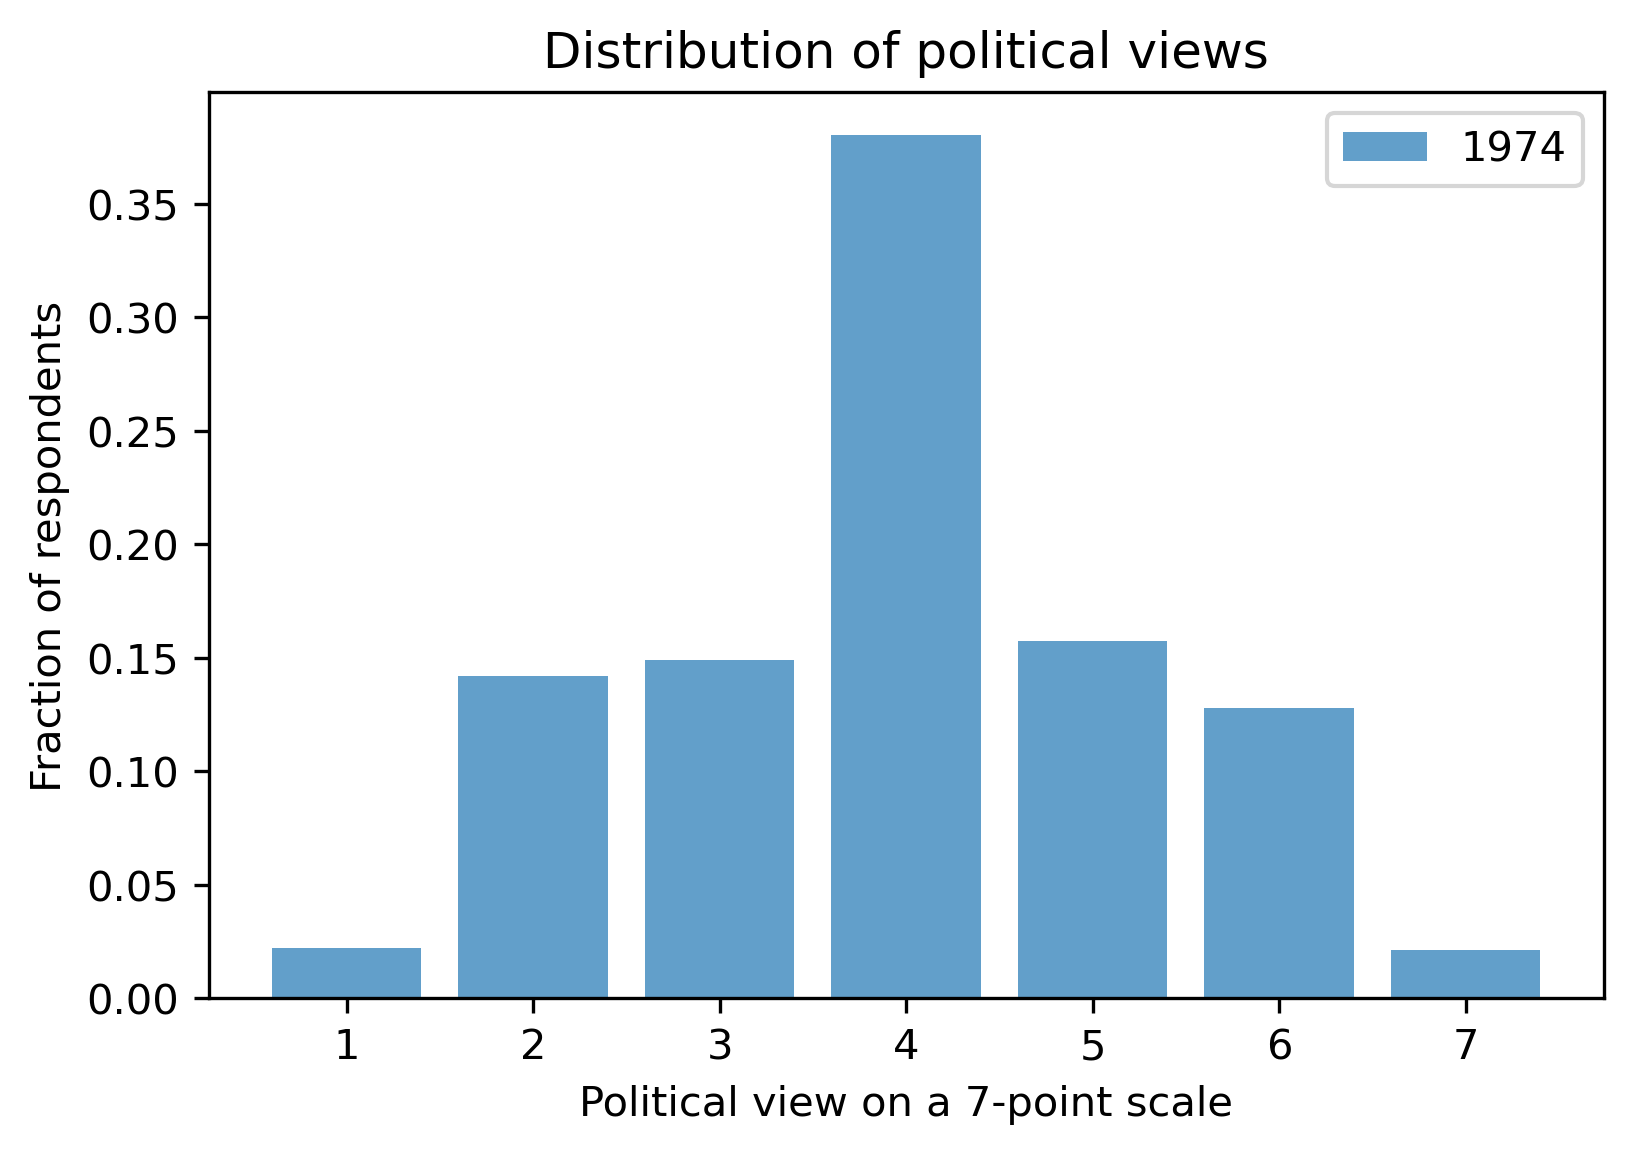
\includegraphics[scale=0.75]{02_polviews_files/02_polviews_32_0.png}
\end{center}

In both cases, the most common response is \passthrough{\lstinline!4!},
which is the code for ``moderate''. And few respondents describe
themselves as ``extremely'' liberal or conservative.

So maybe we're not so polarized after all.

To make it easier to compare the distributions, I'll plot them side by
side.

\begin{lstlisting}[language=Python,style=source]
pmf74.bar(label='1974', width=-0.45, align='edge', alpha=0.7)

pmf18.bar(label='2018', width=0.45, align='edge', alpha=0.7)

decorate(xlabel='Political view on a 7-point scale',
         ylabel='Fraction of population',
         title='Distribution of political views')
\end{lstlisting}

\begin{center}
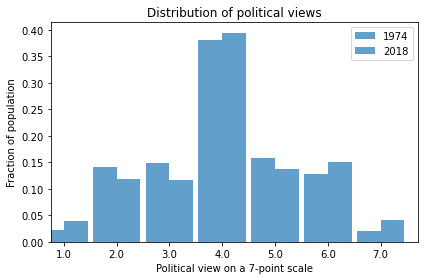
\includegraphics[scale=0.75]{02_polviews_files/02_polviews_34_0.png}
\end{center}

Now we can see the changes in the distribution more clearly. It looks
like the number of people at the extremes (1 and 7) has increased, and
the fraction of liberal (2) and slightly liberal (3) has decreased.

\textbf{Exercise:} To summarize these changes, we can compare the mean
and standard deviation of \passthrough{\lstinline!polviews!} in 1974 and
2018.

The mean of the responses measures the balance of people in the
population with liberal or conservative leanings. If the mean increases
over time, that might indicate a shift in the population toward
conservatism.

The standard deviation measures the dispersion of views in the
population; if it increases over time, that might indicate an increase
in polarization.

Compute the mean and standard deviation of
\passthrough{\lstinline!polviews74!} and
\passthrough{\lstinline!polviews18!}.

What do they indicate about changes over this interval?

\hypertarget{time-series}{%
\section{Time series}\label{time-series}}

At this point we have looked at the endpoints, 1974 and 2018, but we
don't know what happened in between.

To see how the distribution changes over time, we can group by year and
compute the mean of \passthrough{\lstinline!polviews!} during each year.

First I'll use \passthrough{\lstinline!groupby!} to group the
respondents by year.

\begin{lstlisting}[language=Python,style=source]
gss_by_year = gss.groupby('year')
gss_by_year
\end{lstlisting}

\begin{lstlisting}[style=output]
<pandas.core.groupby.generic.DataFrameGroupBy object at 0x7f0788fdc8d0>
\end{lstlisting}

The result is a \passthrough{\lstinline!DataFrameGroupBy!} object that
represents a collection of groups. We can loop through the groups and
display the number of respondents in each:

\begin{lstlisting}[language=Python,style=source]
for year, group in gss_by_year:
    print(year, len(group))
\end{lstlisting}

\begin{lstlisting}[style=output]
1972 1613
1973 1504
1974 1484
1975 1490
1976 1499
1977 1530
1978 1532
1980 1468
1982 1860
1983 1599
1984 1473
1985 1534
1986 1470
1987 1819
1988 1481
1989 1537
1990 1372
1991 1517
1993 1606
1994 2992
1996 2904
1998 2832
2000 2817
2002 2765
2004 2812
2006 4510
2008 2023
2010 2044
2012 1974
2014 2538
2016 2867
2018 2348
\end{lstlisting}

In many ways the \passthrough{\lstinline!DataFrameGroupBy!} behaves like
a \passthrough{\lstinline!DataFrame!}. We can use the bracket operator
to select a column:

\begin{lstlisting}[language=Python,style=source]
polviews_by_year = gss_by_year['polviews']
polviews_by_year
\end{lstlisting}

\begin{lstlisting}[style=output]
<pandas.core.groupby.generic.SeriesGroupBy object at 0x7f0788f0a750>
\end{lstlisting}

A column from a \passthrough{\lstinline!DataFrameGroupBy!} is a
\passthrough{\lstinline!SeriesGroupBy!}. If we invoke
\passthrough{\lstinline!mean!} on it, the results is a series that
contains the mean of \passthrough{\lstinline!polviews!} for each year of
the survey.

\begin{lstlisting}[language=Python,style=source]
mean_series = polviews_by_year.mean()
\end{lstlisting}

And here's what it looks like.

\begin{lstlisting}[language=Python,style=source]
mean_series.plot(color='C2', label='polviews')
decorate(xlabel='Year', 
         ylabel='Mean (7 point scale)',
         title='Mean of polviews')
\end{lstlisting}

\begin{center}
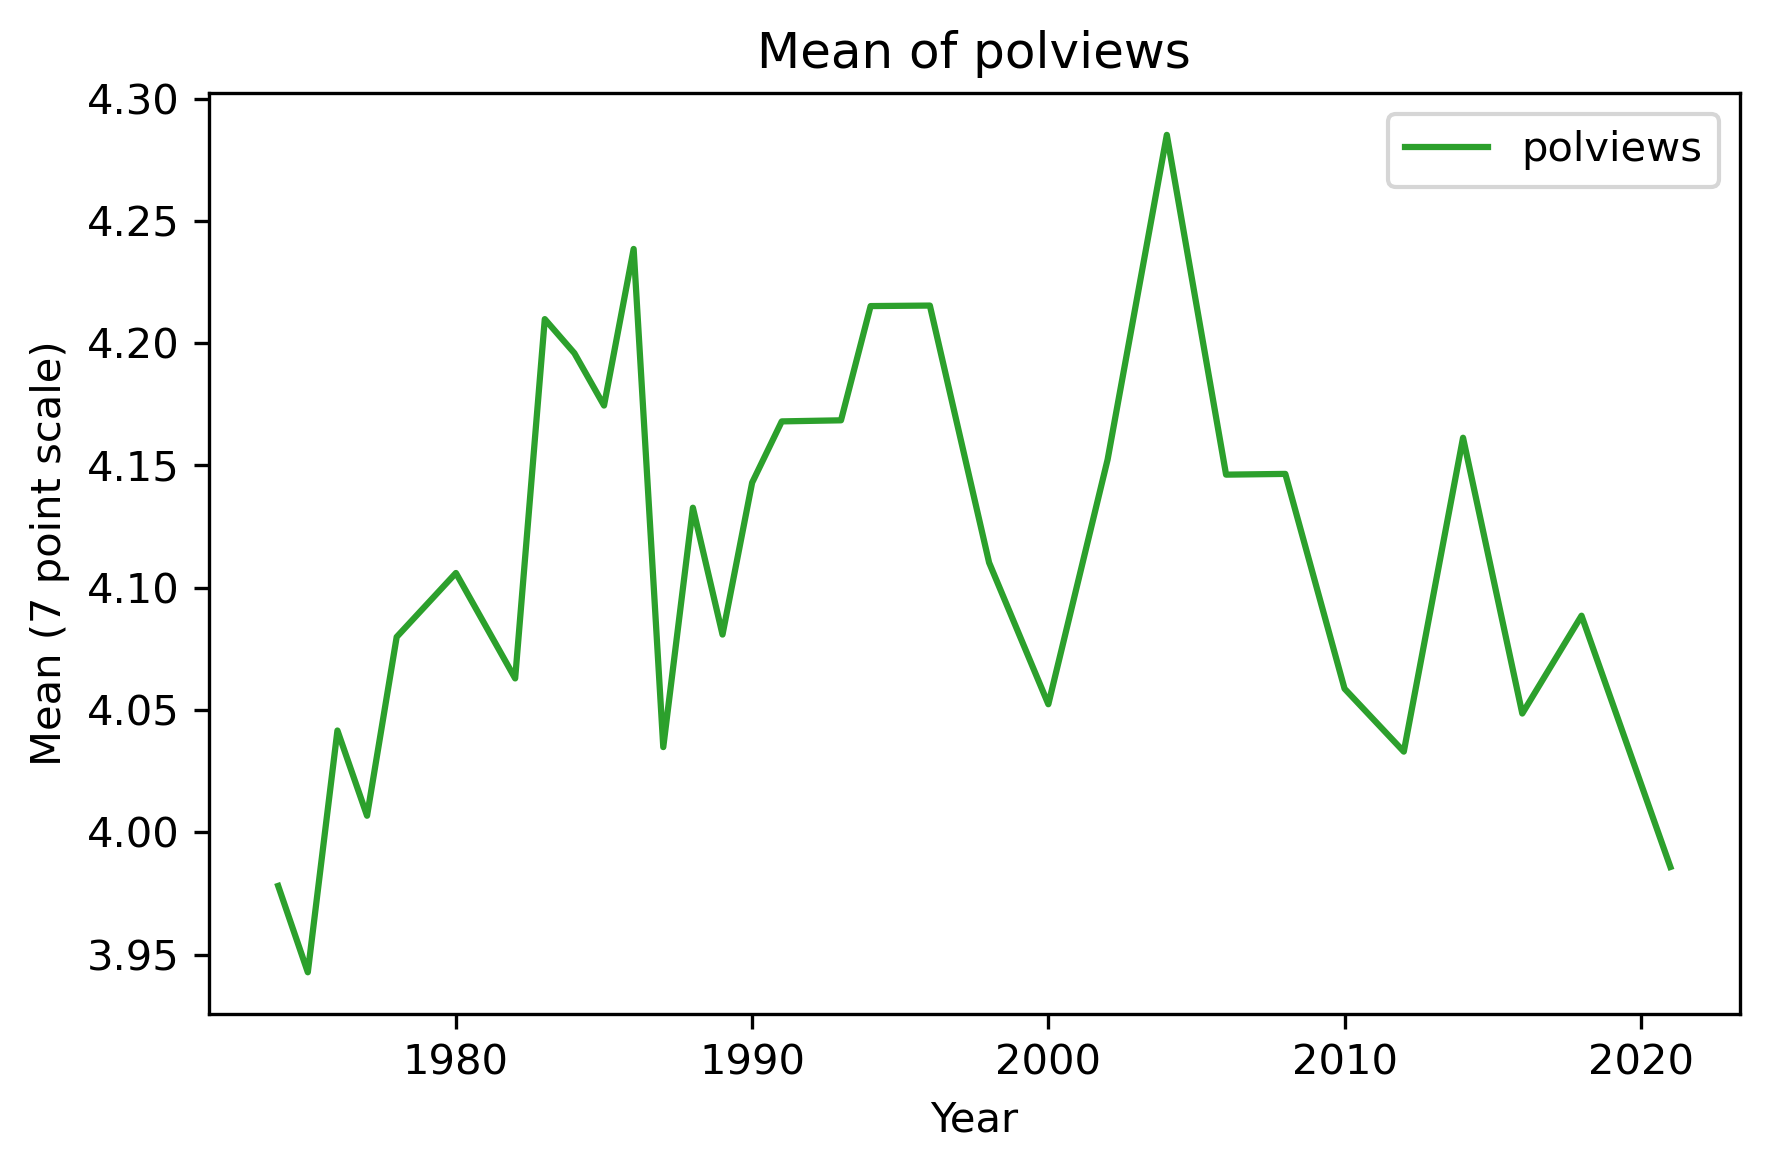
\includegraphics[scale=0.75]{02_polviews_files/02_polviews_46_0.png}
\end{center}

\textbf{Exercise:} The standard deviation quantifies the spread of the
distribution, which is one way to measure polarization.

Plot standard deviation of \passthrough{\lstinline!polviews!} for each
year of the survey from 1972 to 2018.

Does it show evidence of increasing polarization?

\hypertarget{local-regression}{%
\subsection{Local regression}\label{local-regression}}

In the previous section we plotted mean and standard deviation of
\passthrough{\lstinline!polviews!} over time. Both plots are quite
noisy.

We can use \href{https://en.wikipedia.org/wiki/Local_regression}{local
regression} to compute a smooth line through these data points.

The following function takes a Pandas Series and uses and algorithm
called LOWESS to compute a smooth line. LOWESS stands for ``locally
weighted scatterplot smoothing''.

\begin{lstlisting}[language=Python,style=source]
from statsmodels.nonparametric.smoothers_lowess import lowess

def make_lowess(series):
    """Use LOWESS to compute a smooth line.
    
    series: pd.Series
    
    returns: pd.Series
    """
    y = series.values
    x = series.index.values

    smooth = lowess(y, x)
    index, data = np.transpose(smooth)

    return pd.Series(data, index=index) 
\end{lstlisting}

We'll use the following function to plot data points and the smoothed
line.

\begin{lstlisting}[language=Python,style=source]
def plot_series_lowess(series, color):
    """Plots a series of data points and a smooth line.
    
    series: pd.Series
    color: string or tuple
    """
    series.plot(linewidth=0, marker='o', color=color, alpha=0.5)
    smooth = make_lowess(series)
    smooth.plot(label='', color=color)
\end{lstlisting}

The following figure shows the mean of
\passthrough{\lstinline!polviews!} and a smooth line.

\begin{lstlisting}[language=Python,style=source]
mean_series = gss_by_year['polviews'].mean()
plot_series_lowess(mean_series, 'C2')
decorate(ylabel='Mean (7 point scale)',
         title='Mean of polviews',
         xlabel='Year',
         xlim=[1972, 2020])
\end{lstlisting}

\begin{center}
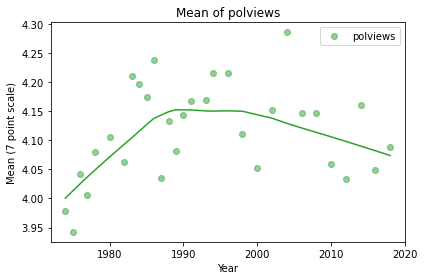
\includegraphics[scale=0.75]{02_polviews_files/02_polviews_53_0.png}
\end{center}

One reason the PMFs for 1974 and 2018 did not look very different is
that the mean seems to have gone up (more conservative) and then down
again (more liberal).

Generally, it looks like the U.S. has been trending toward liberal for
the last 20 years, or more, at least in the sense of how people describe
themselves.

\textbf{Exercise:} Use \passthrough{\lstinline!plot\_series\_lowess!} to
plot the standard deviation of \passthrough{\lstinline!polviews!} with a
smooth line.

\hypertarget{cross-tabulation}{%
\section{Cross tabulation}\label{cross-tabulation}}

In the previous sections, we treated \passthrough{\lstinline!polviews!}
as a numerical quantity, so we were able to compute means and standard
deviations.

But the responses are really categorical, which means that each value
represents a discrete category, like ``liberal'' or ``conservative''.

In this section, we'll treat \passthrough{\lstinline!polviews!} as a
categorical variable. Specifically, we'll compute the number of
respondents in each category for each year, and plot changes over time.

Pandas provides a function called \passthrough{\lstinline!crosstab!}
that computes a
\href{https://en.wikipedia.org/wiki/Contingency_table}{cross
tabulation}.

It takes two Series as arguments and returns a DataFrame.

\begin{lstlisting}[language=Python,style=source]
year = gss['year']
column = gss['polviews']

xtab = pd.crosstab(year, column)
\end{lstlisting}

Here are the first few lines from the result.

\begin{lstlisting}[language=Python,style=source]
xtab.head()
\end{lstlisting}

\begin{tabular}{lrrrrrrr}
\toprule
polviews &  1.0 &  2.0 &  3.0 &  4.0 &  5.0 &  6.0 &  7.0 \\
year &      &      &      &      &      &      &      \\
\midrule
1974 &   31 &  201 &  211 &  538 &  223 &  181 &   30 \\
1975 &   56 &  184 &  207 &  540 &  204 &  162 &   45 \\
1976 &   31 &  198 &  175 &  564 &  209 &  206 &   34 \\
1977 &   37 &  181 &  214 &  594 &  243 &  164 &   42 \\
1978 &   21 &  140 &  255 &  559 &  265 &  187 &   25 \\
\bottomrule
\end{tabular}

It contains one row for each value of \passthrough{\lstinline!year!} and
one column for each value of \passthrough{\lstinline!polviews!}. Reading
the first row, we see that in 1974, 31 people gave response 1,
``extremely liberal'', 201 people gave response 2, ``liberal'', and so
on.

The number of respondents varies from year to year, so we need to
``normalize'' the results, which means computing for each year the
\emph{fraction} of respondents in each category, rather than the count.

\passthrough{\lstinline!crosstab!} takes an optional argument that
normalizes each row.

\begin{lstlisting}[language=Python,style=source]
xtab_norm = pd.crosstab(year, column, normalize='index')
\end{lstlisting}

Here's what that looks like for the 7-point scale.

\begin{lstlisting}[language=Python,style=source]
xtab_norm.head()
\end{lstlisting}

\begin{tabular}{lrrrrrrr}
\toprule
polviews &       1.0 &       2.0 &       3.0 &       4.0 &       5.0 &       6.0 &       7.0 \\
year &           &           &           &           &           &           &           \\
\midrule
1974 &  0.021908 &  0.142049 &  0.149117 &  0.380212 &  0.157597 &  0.127915 &  0.021201 \\
1975 &  0.040057 &  0.131617 &  0.148069 &  0.386266 &  0.145923 &  0.115880 &  0.032189 \\
1976 &  0.021877 &  0.139732 &  0.123500 &  0.398024 &  0.147495 &  0.145378 &  0.023994 \\
1977 &  0.025085 &  0.122712 &  0.145085 &  0.402712 &  0.164746 &  0.111186 &  0.028475 \\
1978 &  0.014463 &  0.096419 &  0.175620 &  0.384986 &  0.182507 &  0.128788 &  0.017218 \\
\bottomrule
\end{tabular}

To make the results easier to interpret, I'm going to replace the
numeric codes 1-7 with strings. First I'll make a dictionary that maps
from numbers to strings:

\begin{lstlisting}[language=Python,style=source]
# recode the 7 point scale with words
d7 = {1: 'Extremely liberal', 
      2: 'Liberal', 
      3: 'Slightly liberal', 
      4: 'Moderate', 
      5: 'Slightly conservative', 
      6: 'Conservative', 
      7: 'Extremely conservative'}
\end{lstlisting}

Then we can use the \passthrough{\lstinline!replace!} function like
this:

\begin{lstlisting}[language=Python,style=source]
polviews7 = gss['polviews'].replace(d7)
\end{lstlisting}

We can use \passthrough{\lstinline!values!} to confirm that the values
in \passthrough{\lstinline!polviews7!} are strings.

\begin{lstlisting}[language=Python,style=source]
values(polviews7)
\end{lstlisting}

\begin{tabular}{lr}
\toprule
{} &  polviews \\
\midrule
Conservative           &      8495 \\
Extremely conservative &      1770 \\
Extremely liberal      &      1699 \\
Liberal                &      6299 \\
Moderate               &     21444 \\
Slightly conservative  &      8864 \\
Slightly liberal       &      6981 \\
\bottomrule
\end{tabular}

If we make the cross tabulation again, we can see that the column names
are strings.

\begin{lstlisting}[language=Python,style=source]
xtab_norm = pd.crosstab(year, polviews7, normalize='index')
xtab_norm.head()
\end{lstlisting}

\begin{tabular}{lrrrrrrr}
\toprule
polviews &  Conservative &  Extremely conservative &  Extremely liberal &   Liberal &  Moderate &  Slightly conservative &  Slightly liberal \\
year &               &                         &                    &           &           &                        &                   \\
\midrule
1974 &      0.127915 &                0.021201 &           0.021908 &  0.142049 &  0.380212 &               0.157597 &          0.149117 \\
1975 &      0.115880 &                0.032189 &           0.040057 &  0.131617 &  0.386266 &               0.145923 &          0.148069 \\
1976 &      0.145378 &                0.023994 &           0.021877 &  0.139732 &  0.398024 &               0.147495 &          0.123500 \\
1977 &      0.111186 &                0.028475 &           0.025085 &  0.122712 &  0.402712 &               0.164746 &          0.145085 \\
1978 &      0.128788 &                0.017218 &           0.014463 &  0.096419 &  0.384986 &               0.182507 &          0.175620 \\
\bottomrule
\end{tabular}

We are almost ready to plot the results, but first we need some colors.

\hypertarget{color-palettes}{%
\section{Color palettes}\label{color-palettes}}

Seaborn provides a variety of color palettes,
\href{https://seaborn.pydata.org/tutorial/color_palettes.html}{which you
can read about here}.

To represent political views, I'll use a diverging palette from blue to
red.

\begin{lstlisting}[language=Python,style=source]
palette = sns.color_palette('RdBu_r', 7)
sns.palplot(palette)
\end{lstlisting}

\begin{center}
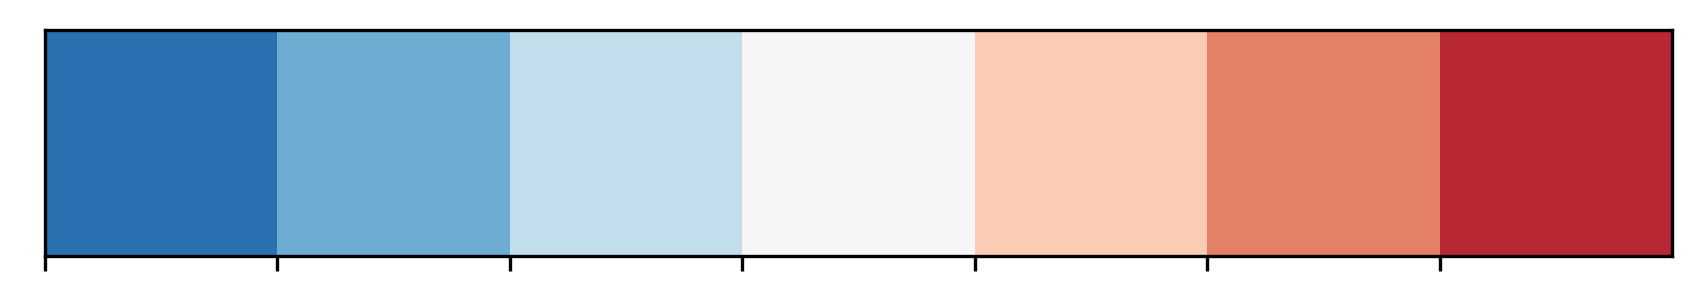
\includegraphics[scale=0.75]{02_polviews_files/02_polviews_74_0.png}
\end{center}

The middle color is white, which won't work when we plot it, so I will
replace it with a purple color from another palette.

\begin{lstlisting}[language=Python,style=source]
muted = sns.color_palette('muted', 7)
purple = muted[4]
sns.palplot(muted)
\end{lstlisting}

\begin{center}
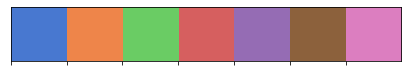
\includegraphics[scale=0.75]{02_polviews_files/02_polviews_76_0.png}
\end{center}

Here's the modified diverging palette with purple in the middle.

\begin{lstlisting}[language=Python,style=source]
palette[3] = purple
sns.palplot(palette)
\end{lstlisting}

\begin{center}
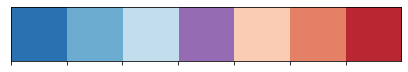
\includegraphics[scale=0.75]{02_polviews_files/02_polviews_78_0.png}
\end{center}

A feature of this color map is that the colors are meaningful, at least
in countries that use blue, purple, and red for these points on the
political spectrum. A drawback of this color map is that some some of
the colors are indistinguishable to people who are
\href{https://davidmathlogic.com/colorblind}{color blind}.

Now I'll make a dictionary that maps from the responses to the
corresponding colors.

\begin{lstlisting}[language=Python,style=source]
columns = ['Extremely liberal', 
           'Liberal', 
           'Slightly liberal', 
           'Moderate', 
           'Slightly conservative', 
           'Conservative',
           'Extremely conservative']
\end{lstlisting}

\begin{lstlisting}[language=Python,style=source]
color_map = dict(zip(columns, palette))

for key, value in color_map.items():
    print(key, value)
\end{lstlisting}

\begin{lstlisting}[style=output]
Extremely liberal (0.16339869281045757, 0.44498269896193776, 0.6975009611687812)
Liberal (0.4206843521722416, 0.6764321414840447, 0.8186851211072664)
Slightly liberal (0.7614763552479817, 0.8685121107266438, 0.924567474048443)
Moderate (0.5843137254901961, 0.4235294117647059, 0.7058823529411765)
Slightly conservative (0.9824682814302191, 0.8006920415224913, 0.7061130334486736)
Conservative (0.8945790080738177, 0.5038062283737024, 0.39976931949250283)
Extremely conservative (0.7284890426758939, 0.15501730103806227, 0.1973856209150327)
\end{lstlisting}

\hypertarget{plotting}{%
\section{Plotting}\label{plotting}}

To plot the results, I use the following function, which takes a
\passthrough{\lstinline!DataFrame!} and plots each column using
\passthrough{\lstinline!plot\_series\_lowess!}.

\begin{lstlisting}[language=Python,style=source]
def plot_columns_lowess(table, columns, colors):
    """Plot the columns in a DataFrame.
    
    table: DataFrame with a cross tabulation
    columns: list of column names, in the desired order
    colors: mapping from column names to colors
    """
    for col in columns:
        series = table[col]
        plot_series_lowess(series, colors[col])
\end{lstlisting}

The following function sets the position of the figure legend.

\begin{lstlisting}[language=Python,style=source]
def anchor_legend(x, y):
    """Place the upper left corner of the legend box.
    
    x: x coordinate
    y: y coordinate
    """
    plt.legend(bbox_to_anchor=(x, y), loc='upper left', ncol=1)
\end{lstlisting}

Here are the 7 categories plotted as a function of time.

\begin{lstlisting}[language=Python,style=source]
plot_columns_lowess(xtab_norm, columns, color_map)
decorate(xlabel='Year',
         ylabel='Proportion',
         title='Fraction of people with each political view',
         xlim=[1972, 2020])

anchor_legend(1.02, 1.02)
\end{lstlisting}

\begin{center}
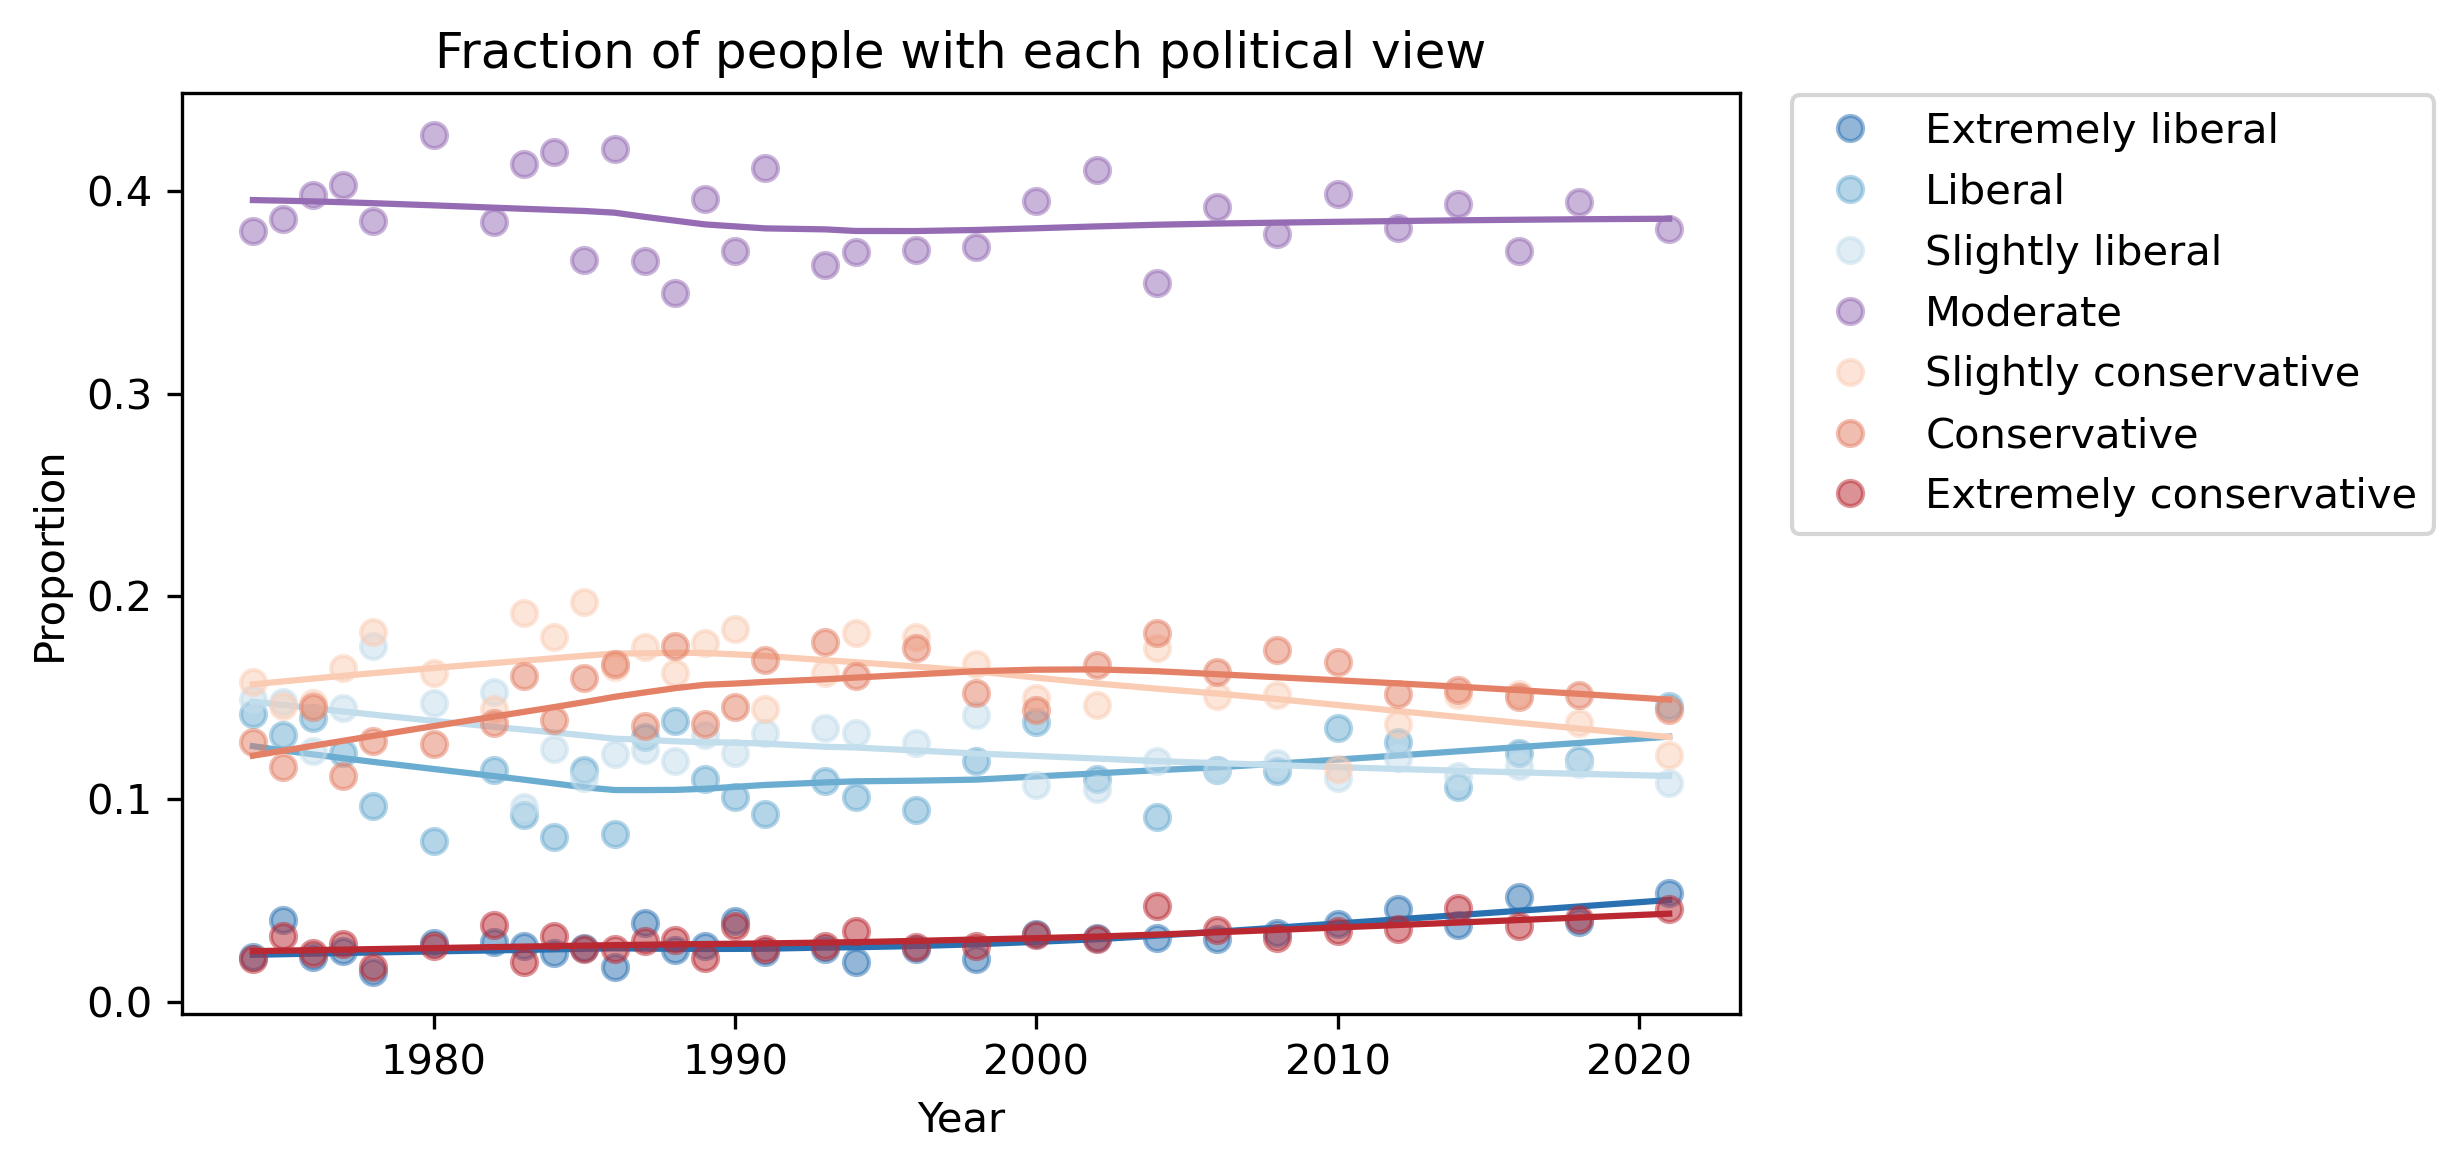
\includegraphics[scale=0.75]{02_polviews_files/02_polviews_87_0.png}
\end{center}

This way of looking at the results suggests that changes in political
alignment during this period have generally been slow and small.

The fraction of self-described moderates has not changed substantially.

The fraction of conservatives increased, but seems to be decreasing now;
the number of liberals seems to be increasing.

The fraction of people at the extremes has increased, but it is hard to
see clearly in this figure.

We can get a better view by plotting just the extremes.

\begin{lstlisting}[language=Python,style=source]
columns2 = ['Extremely liberal', 'Extremely conservative']

plot_columns_lowess(xtab_norm, columns2, color_map)
decorate(xlabel='Year',
         ylabel='Proportion',
         title='Fraction of people with extreme political views',
         xlim=[1970, 2020])

anchor_legend(1.02, 1.02)
\end{lstlisting}

\begin{center}
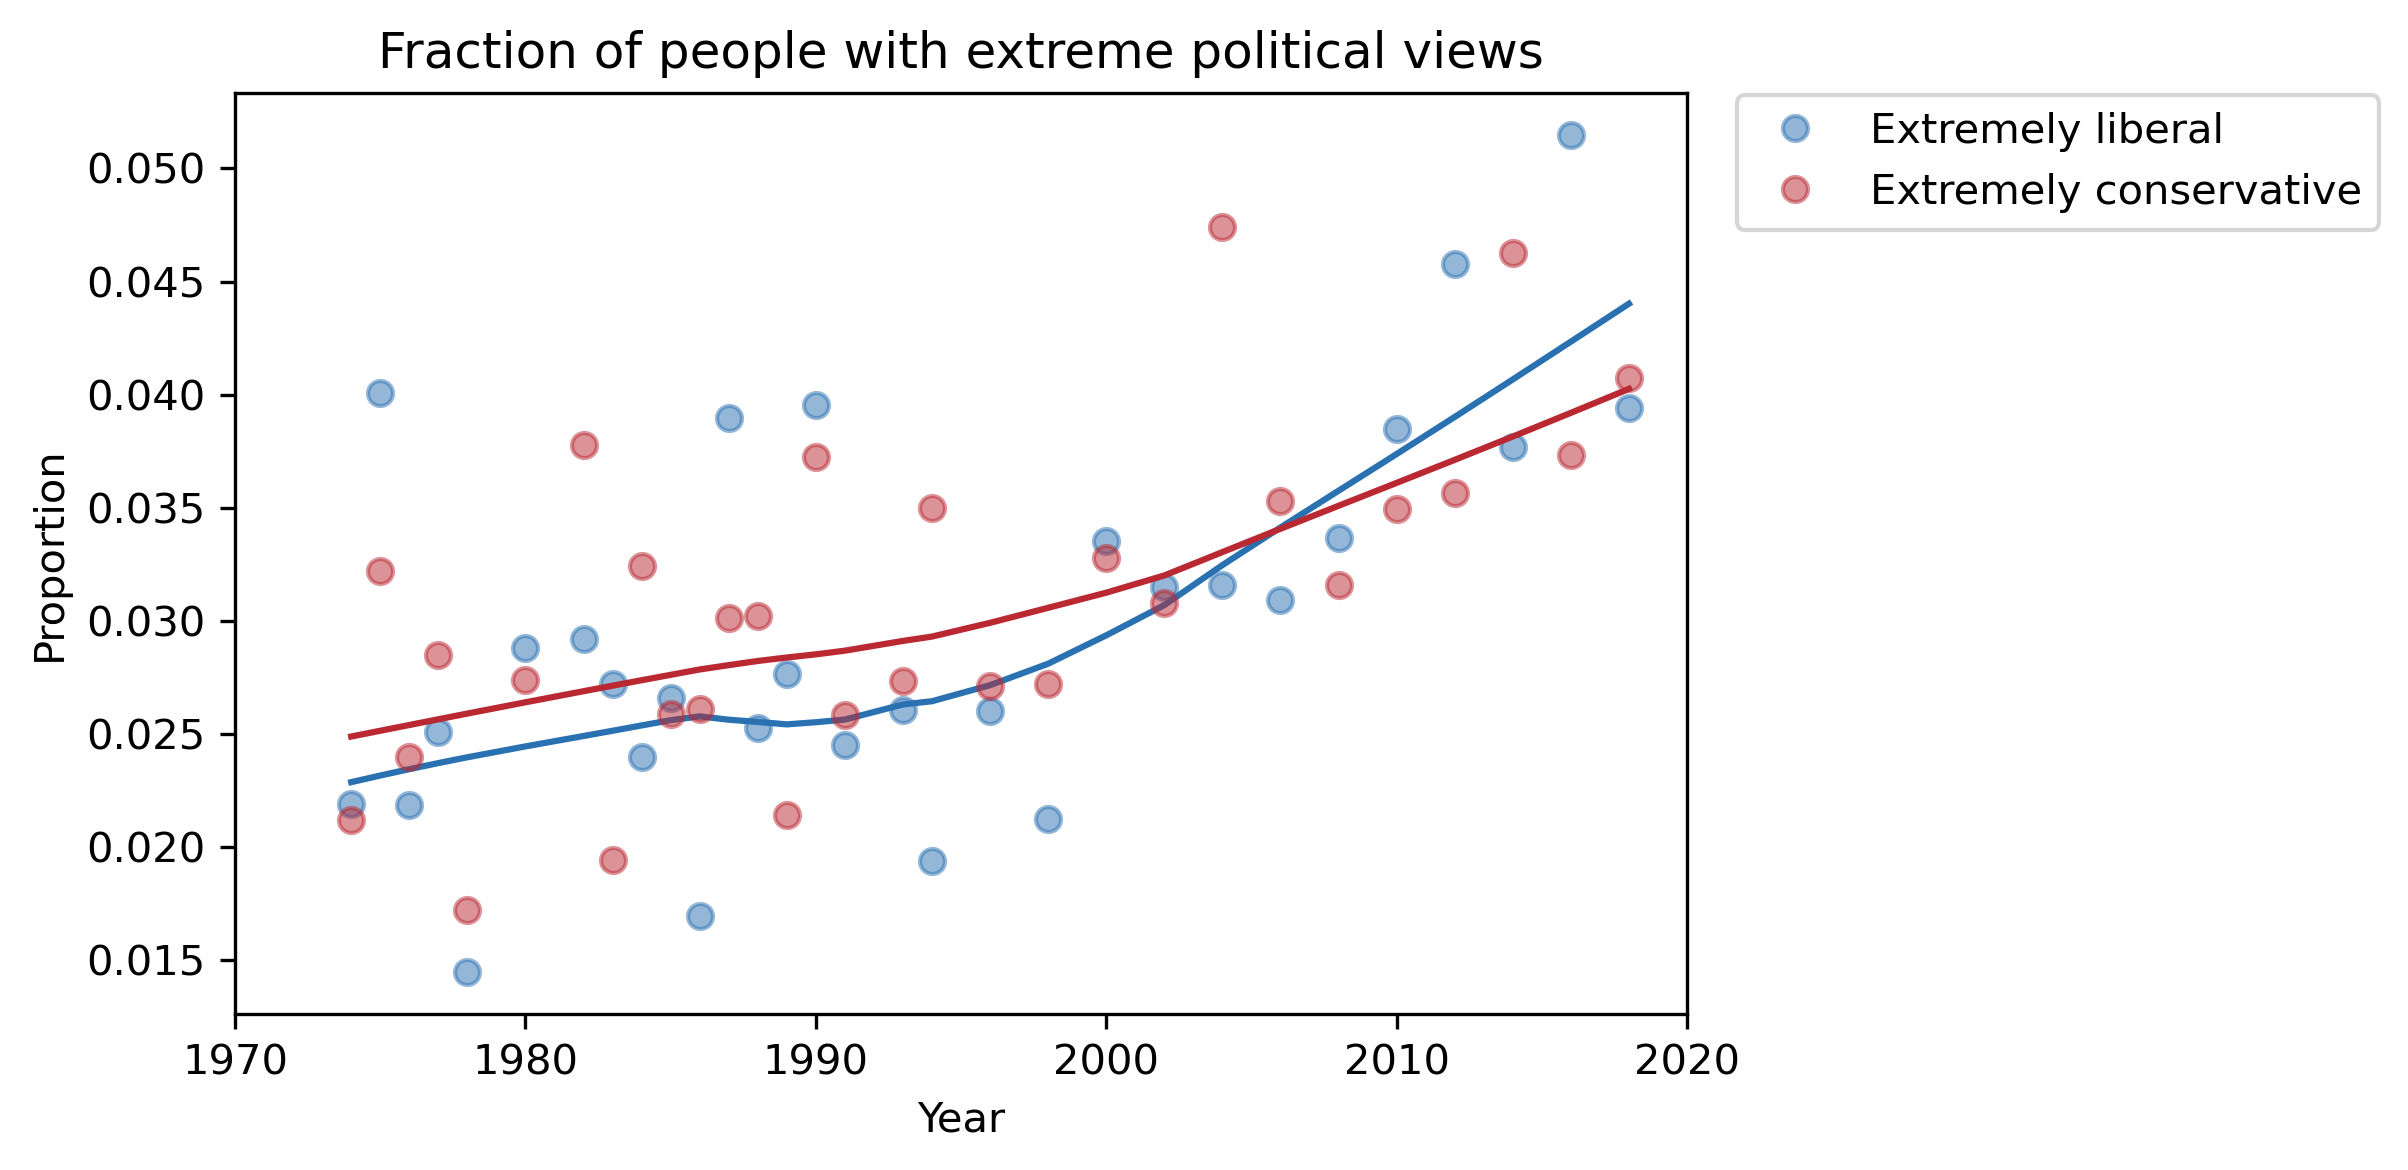
\includegraphics[scale=0.75]{02_polviews_files/02_polviews_89_0.png}
\end{center}

This figure shows that the fraction of people who describe themselves as
``extreme'' has increased from about 2.5\% to about 4\%.

In relative terms, that's a big increase. But in absolute terms these
tails of the distribution are still small.

\textbf{Exercise:} Let's do a similar analysis with
\passthrough{\lstinline!partyid!}, which encodes responses to the
question:

\begin{quote}
Generally speaking, do you usually think of yourself as a Republican,
Democrat, Independent, or what?
\end{quote}

The valid responses are:

\begin{lstlisting}[style=output]
0   Strong democrat
1   Not str democrat
2   Ind,near dem
3   Independent
4   Ind,near rep
5   Not str republican
6   Strong republican
7   Other party
\end{lstlisting}

You can
\href{https://gssdataexplorer.norc.org/projects/52787/variables/141/vshow}{read
the codebook for \passthrough{\lstinline!partyid!} here}.

Here are the steps I suggest:

\begin{enumerate}
\def\labelenumi{\arabic{enumi})}
\item
  If you have not already saved this notebook, you should do that first.
  If you are running on Colab, select ``Save a copy in Drive'' from the
  File menu.
\item
  Now, before you modify this notebook, make \emph{another} copy and
  give it an appropriate name.
\item
  Search and replace \passthrough{\lstinline!polviews!} with
  \passthrough{\lstinline!partyid!} (use ``Edit-\textgreater Find and
  replace'').
\item
  Run the notebook from the beginning and see what other changes you
  have to make.
\end{enumerate}

You will have to make changes in \passthrough{\lstinline!d7!} and
\passthrough{\lstinline!columns!}. Otherwise you might get a message
like

\passthrough{\lstinline!TypeError: '<' not supported between instances of 'float' and 'str'!}

Also, you might have to drop ``Other party'' or change the color
palette.

And you should change the titles of the figures.

What changes in party affiliation do you see over the last 50 years? Are
things going in the directions you expected?

Write a headline (or a couple) that describe the most substantial
changes you see.

